
\begin{figure}[h]
    \centering
    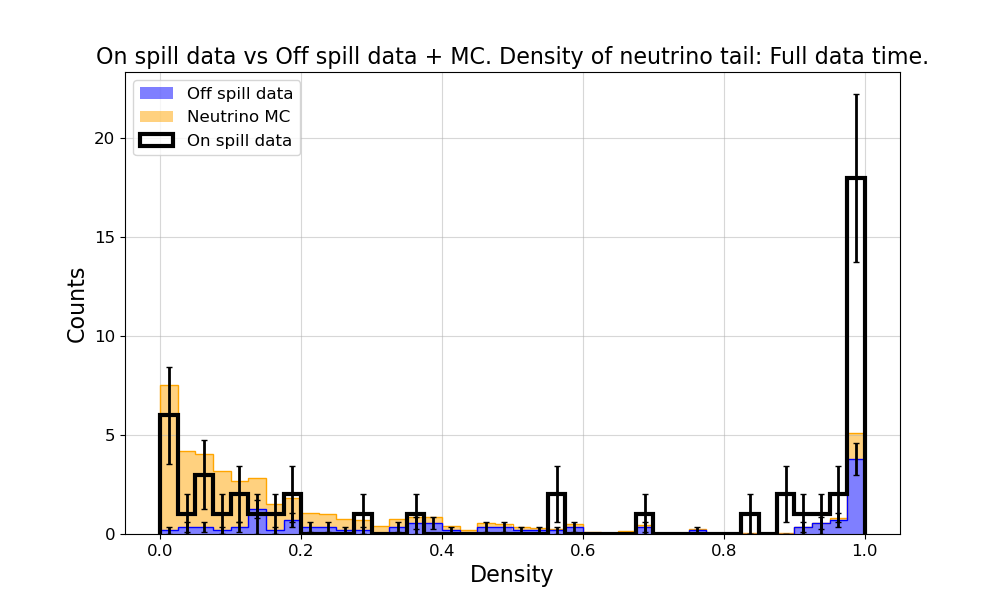
\includegraphics[width=0.69\linewidth]{sections/plots/version_1/beam_on_vs_off/full_time_high_tps/sig_bkg_mc_tail_density_full_sig_time.png}
    \caption{Tail density distribution comparing beam-on data with the stacked distributions of beam-off and Monte Carlo neutrinos.}
    \label{fig:high_tps_beam_on_tail_density_v1}
\end{figure}

\begin{figure}[h]
    \centering
    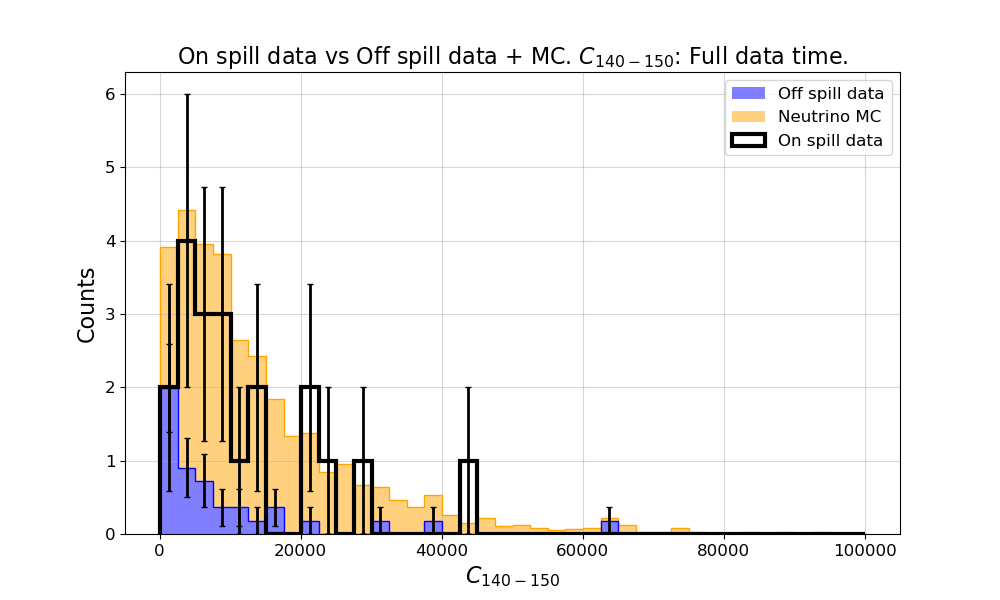
\includegraphics[width=0.69\linewidth]{sections/plots/version_1/beam_on_vs_off/full_time_high_tps/sig_bkg_mc_energyDepositedInFifteenth10cm_spectrum_full_sig_time.png}
    \caption{Charge deposited in the fifteenth 10~cm bin comparing beam-on data with the stacked distributions of beam-off and Monte Carlo neutrinos.}
    \label{fig:high_tps_beam_on_energyDepositedInFifteenth10cm_v1}
\end{figure}

\begin{figure}[h]
    \centering
    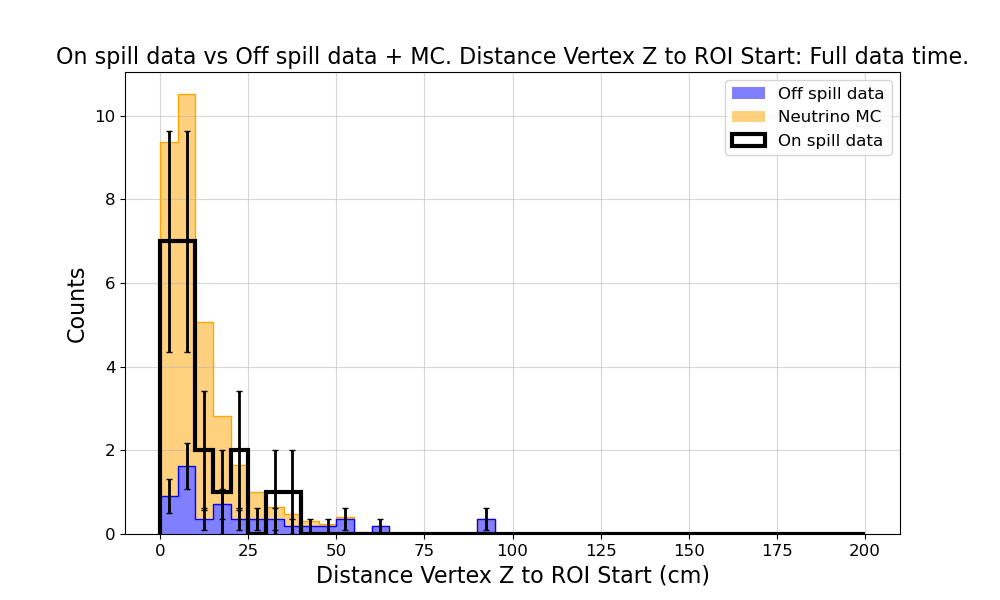
\includegraphics[width=0.69\linewidth]{sections/plots/version_1/beam_on_vs_off/full_time_high_tps/sig_bkg_mc_distance_vertexZ_to_ROI_start_full_sig_time.png}
    \caption{Distance from vertex Z to ROI start comparing beam-on data with the stacked distributions of beam-off and Monte Carlo neutrinos.}
    \label{fig:high_tps_beam_on_distance_vertexZ_to_ROI_start_v1}
\end{figure}

\begin{figure}[h]
    \centering
    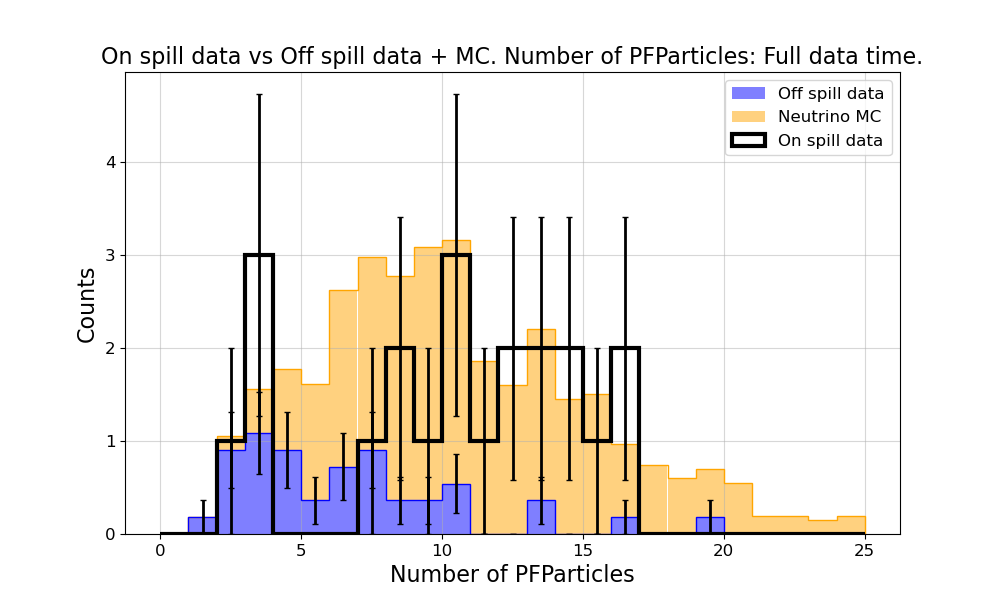
\includegraphics[width=0.69\linewidth]{sections/plots/version_1/beam_on_vs_off/full_time_high_tps/sig_bkg_mc_numberOfPFParticles_spectrum_full_sig_time.png}
    \caption{Number of PFParticles comparing beam-on data with the stacked distributions of beam-off and Monte Carlo neutrinos.}
    \label{fig:high_tps_beam_on_numberOfPFParticles_v1}
\end{figure}

\begin{figure}[h]
    \centering
    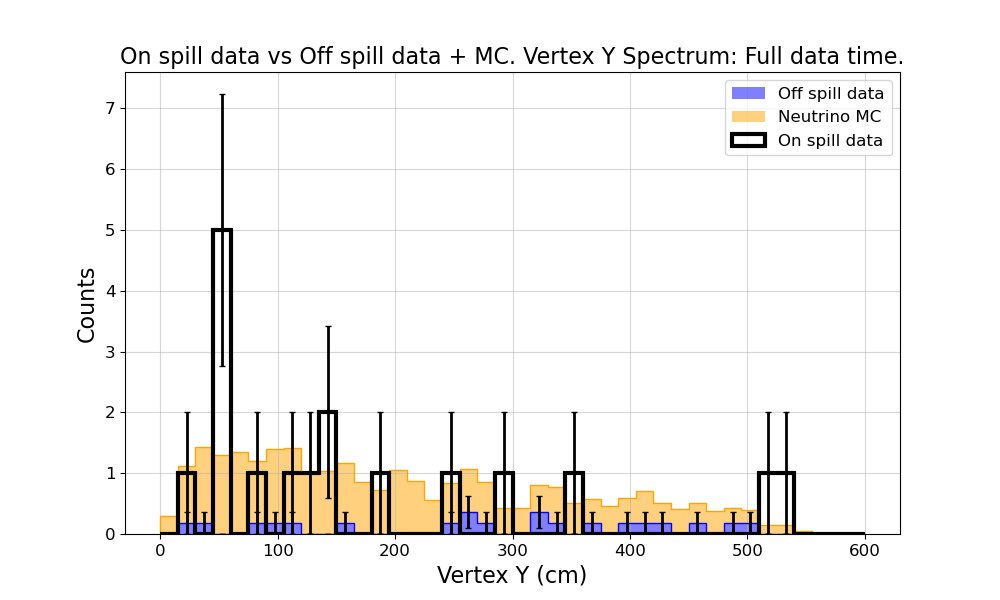
\includegraphics[width=0.69\linewidth]{sections/plots/version_1/beam_on_vs_off/full_time_high_tps/sig_bkg_mc_vertexY_spectrum_full_sig_time.png}
    \caption{Vertex Y position comparing beam-on data with the stacked distributions of beam-off and Monte Carlo neutrinos.}
    \label{fig:high_tps_beam_on_vertexY_v1}
\end{figure}

\begin{figure}[h]
    \centering
    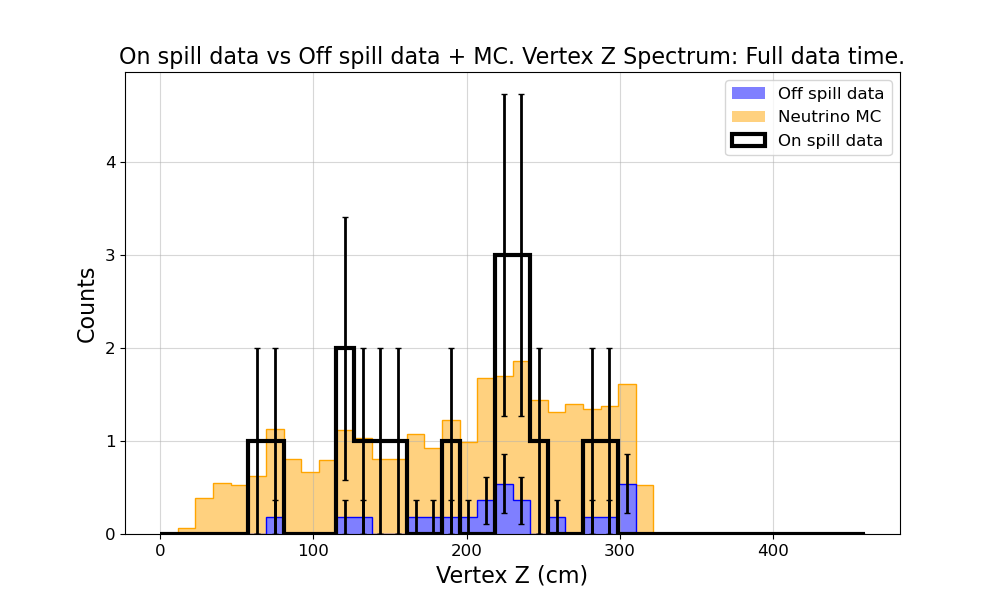
\includegraphics[width=0.69\linewidth]{sections/plots/version_1/beam_on_vs_off/full_time_high_tps/sig_bkg_mc_vertexZ_spectrum_full_sig_time.png}
    \caption{Vertex Z position comparing beam-on data with the stacked distributions of beam-off and Monte Carlo neutrinos.}
    \label{fig:high_tps_beam_on_vertexZ_v1}
\end{figure}

\begin{figure}[h]
    \centering
    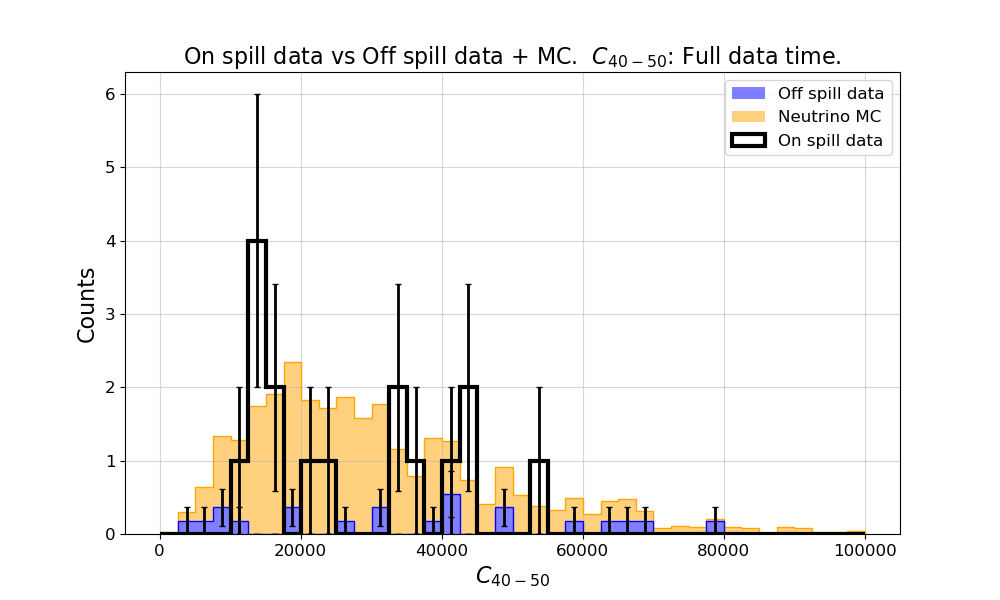
\includegraphics[width=0.69\linewidth]{sections/plots/version_1/beam_on_vs_off/full_time_high_tps/sig_bkg_mc_energyDepositedInFifth10cm_spectrum_full_sig_time.png}
    \caption{Charge deposited in the fifth 10~cm bin comparing beam-on data with the stacked distributions of beam-off and Monte Carlo neutrinos.}
    \label{fig:high_tps_beam_on_energyDepositedInFifth10cm_v1}
\end{figure}

\begin{figure}[h]
    \centering
    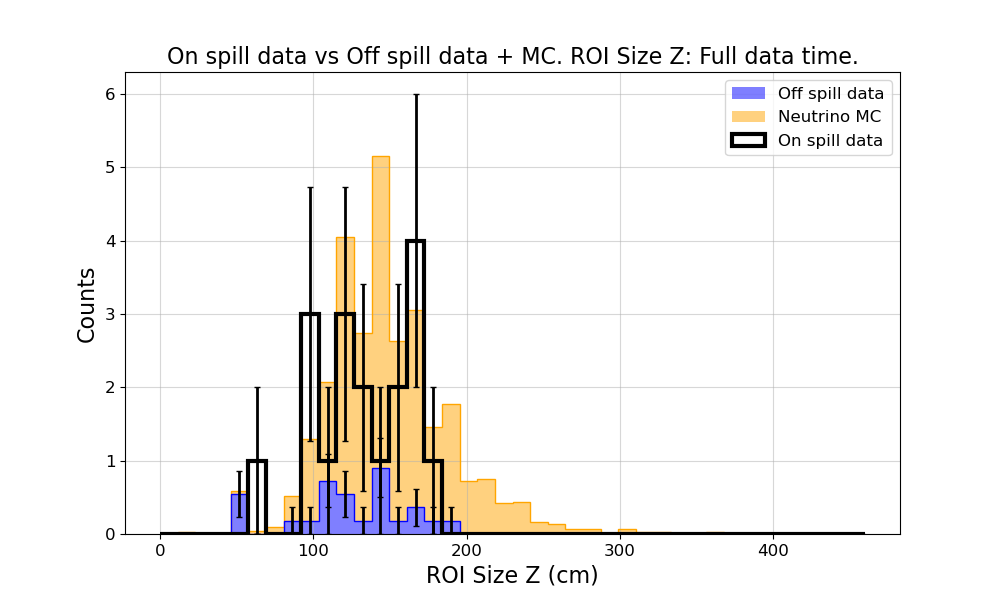
\includegraphics[width=0.69\linewidth]{sections/plots/version_1/beam_on_vs_off/full_time_high_tps/sig_bkg_mc_ROI_Z_size_spectrum_full_sig_time.png}
    \caption{ROI Z size spectrum comparing beam-on data with the stacked distributions of beam-off and Monte Carlo neutrinos.}
    \label{fig:high_tps_beam_on_ROI_Z_size_v1}
\end{figure}

\begin{figure}[h]
    \centering
    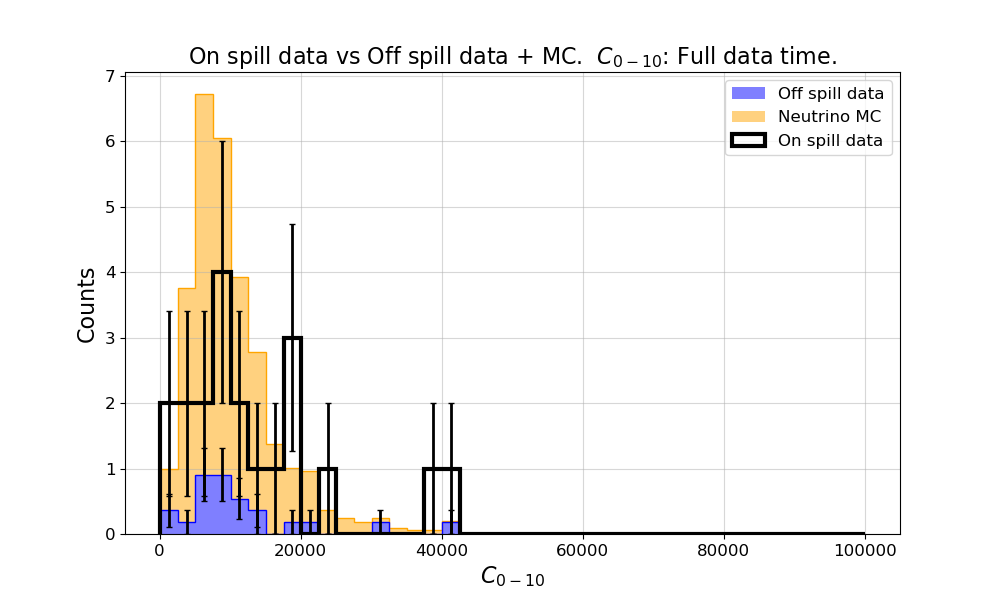
\includegraphics[width=0.69\linewidth]{sections/plots/version_1/beam_on_vs_off/full_time_high_tps/sig_bkg_mc_energyDepositedInFirst10cm_spectrum_full_sig_time.png}
    \caption{Charge deposited in the first 10~cm bin comparing beam-on data with the stacked distributions of beam-off and Monte Carlo neutrinos.}
    \label{fig:high_tps_beam_on_energyDepositedInFirst10cm_v1}
\end{figure}
